\chapter{Audio Synthesizers}
\label{chapter:background}

\graphicspath{{./}{./figures/}{./figures/background/}}

Martin Russ introduces the synthesizer as any device that generates sound \cite{russ2012sound}.  Even the human voice can be thought of as a synthesizer. However, sound synthesizers have become more broadly accepted as an electronic musical instrument that produces synthetic sounds. A synthesizer may do this through playback and recombining preexisting audio or through generating and shaping raw audio waveforms. Numerous types of synthesis techniques exist and are capable of producing a significant variety of sounds.

%Broadly speaking, the sounds that a synthesizer generates can be categorized into two different classes: `imitative` or `synthetic`. Imitative sounds attempt to emulate a sound that exists in the natural world such as a physical musical instrument or a sound effect and synthetic sounds are those that have no relation to a sound in the physical world. The distinction between imitative and synthetic sounds is blurry and most sounds fall somewhere in the middle. Designing new sounds, whether they are imitative, synthetic, or somewhere in between, involves adjusting 

This chapter serves as background for audio synthesizers to provide context and motivation for research focused on improving their usability. Section \ref{section:synth-history} describes the evolution of synthesizers and provides historical context for developments in synthesizer technology relevant to this thesis. Section \ref{section:synth-anatomy} overviews some of the main components of a typical synthesizer and introduces two of the most common types of synthesis: subtractive and frequency modulation (FM) synthesis. Section \ref{section:synth-programming} introduces the topic of synthesizer programming in more depth and discusses the associated challenges and opportunities for improvement.

% Broadly speaking, these sounds can be categorized into two different classes: `imitative` or `synthetic`. Imitative sounds attempt to emulate a sound that exists in the natural world such as a physical musical instrument or a sound effect such as an explosion. Electric pianos are examples of imitative synthesizers. Synthetic sounds are those that have no relation to a sound in the physical world. The distinction between imitative and synthetic sounds is blurry and most sounds fall somewhere in the middle. For example, synth-brass sounds, which were a staple of synths such as Roland's popular Jupiter-8, are sounds that are based on an imitation of a brass sound but extend into the synthetic realm.


\section{Evolution of Synthesizers}
\label{section:synth-history}
% A brief history of the development and use of synthesizers is provided here for historical context. The full history of the topic is beyond the scope of this thesis and the interested reader is referred to some great textbooks that cover audio synthesizers and their history \cite{roads1980interview, mcguire2015musical, jenkins2019analog, russ2012sound}, which were used in the writing of this chapter.
\subsection{Analog Synthesizers}
Until the late 1950s all synthesizers were analog. Analog synthesizers are defined by their use of continuous-time signals, as opposed to digital synthesizers, which use discrete-time signals (or signals consisting of separate, discrete pieces of information). Early analog synthesizers can be broken down into two broad categories based on their approach to sound generation: (1) sounds are generated directly by electric circuits or oscillating vacuum tubes, or (2) sounds are generated by rotating or vibrating physical systems that are controlled by electronic sources \cite{roads1996computer}. The first -- and the largest -- sound synthesizer ever built was developed in the early 1900s by Thaddeus Cahill. On September 26, 1906, an audience of 900 individuals gathered to view the massive electronic instrument, called the Telharmonium, that was capable of producing pure sinusoidal waves, which was sound that had never been heard before. Other early synthesizers include the Theremin, built by Leon Theremin in 1920, which produced a pure tone with a varying pitch and amplitude that is controlled by a performer moving their arms in relation to two antennas. Versions of the theremin have been used in popular music by musicians including The Beach Boys, Led Zeppelin, and The Rolling Stones. %The Ondes Martenot, developed in 1928 by Maurice Martenot and Ondes, had a similar sound to the theremin and also was one of the first synthesizers to include a piano-like keyboard interface.

In the 1960s, two companies emerged on opposite sides of America and released synthesizers that shaped the modern landscape of audio synthesis. Around 1964, Don Buchla, who lived in the San Francisco area, released the the Buchla 100 Series Modular Electronic Music System. At the same time, in New York, Robert Moog released the R.A. Moog Modular System \cite{mcguire2015musical}. Both synthesizers were modular systems containing individual processing units called \textit{modules} that could be interconnected using patch cables. Connecting together synthesizer modules is known as creating a \textit{synth patch}, or simply a \textit{patch}. Both the Buchla and Moog systems introduced Voltage-Controlled Oscillators (VCOs) which created electronic waveforms at musical pitches and could be controlled using an input signal called a control-voltage (CV). The Moog Modular System also featured a Voltage Controlled Filter (VCF) that was an early version of Moog's famous ladder filter design. This filter could resonate at a controllable frequency and was responsible for creating some of the most iconic synthesizer sounds that are still heard in contemporary music.

Important philosophical differences between Moog and Buchla Synthesizers lead to two distinct schools of thought: East Coast and West Coast synthesis. The development of the Buchla synthesizer by Don Buchla was guided by Morton Subotnick and other experimental composers working out of the San Francisco Tape Music Center. Subotnick explicitly requested that the synthesizer was not to be controlled by a traditional keyboard interface as he was worried that it would trap him into creating traditional tonal music. Instead, Buchla synthesizers are controlled using a set of touch plates and sequencers. At the same time, on the East coast, Robert Moog was developing the Moog Modular, which featured a traditional keyboard interface. This allowed the Moog Modular Systems to be integrated more easily with Western music and was one of the reasons that Moog synthesizers became much more popular and commercially successful compared to Buchla synthesizers. 

Another reason that Moog synthesizers were launched into the public eye was due to  their use in recorded music. In 1968 Wendy Carlos used a Moog Modular synthesizer to orchestrate, perform, and record a selection of Johann Sebastian Bach pieces. The collection of music, called \textit{Switched On Bach}, went on to become the best selling classical recording of all time. Other musicians had recreated classical music pieces on synthesizers, but none had reached the same level as \textit{Switch On Bach}. The success of the release was in part attributed to Carlos' ability to design synthesizer sounds that worked synergistically with Bach's compositions \cite{jenkins2019analog}. Building on this success, Carlos went on to score synthesized soundtracks for movies including Stanley Kubrick's \textit{A Clockwork Orange}. Another exceptional example of classical music recreated using Moog synthesizers is Japanese composer Isao Tomita's \textit{Snowflakes Are Dancing}, which was released in 1974. The use of synthesizers in music and film extends into almost all genres of music and was the cornerstone in the development of new genres including techno and other electronic music genres. For more information, see Mark Jenkins' overview of the use of synthesizers throughout different genres of music in his book \textit{Analog Synthesizers: Understanding, Performing, Buying} \cite{jenkins2019analog}.

\subsection{Digital Synthesizers}
The first experiments with digital synthesis were conducted by Max Mathews on an IBM 704 computer in 1957 \cite{roads1980interview}. These experiments consisted of programming and synthesizing melodies using simple waveforms. The Music III program was developed by Mathews in 1960 and introduced an important concept called the \textit{unit generator}, which was used to define basic components of a synthesizer that could be connected together in a similar way to how one one would ``patch" a modular synthesizer. Mathews describes this concept as being developed in parallel, but separate from similar concepts in the analog synthesizer world (e.g., modular synthesizers). He described this as ``an advantage because a musician who knew who to patch together Moog synthesizer units would have a pretty good idea how to put together unit generators in the computer."

In 1973 John Chowning, a researcher at Stanford, released landmark work on Frequency Modulation (FM) synthesis \cite{chowning1973synthesis}. The patent for FM synthesis was licensed to Yamaha who developed the Yamaha DX7 synthesizer using the technology. After being released in 1983, the Yamaha DX7 became one of the best selling synthesizers of all time. One of the major benefits of FM synthesis is that it can produce complex audio waveforms at low computational cost. Additionally, the Yamaha DX7 was a fully polyphonic synthesizer, which means that it was capable of producing multiple tones simultaneously (i.e., able to play chords), whereas most analog synthesizers at that time were monophonic (or only capable of playing one note at a time). The Yamaha DX7 was also difficult to program, though it came preloaded with a large selection of quality parameter settings, or presets, that allowed users to play the synth without having to learn how to program it. The evidence for the difficulties in using the DX7 have been primarily anecdotal, but ``allegedly, nine out of ten DX7s [that went into] workshops for servicing still had their factory presets intact” \cite{seago2004critical}.

As digital technology improved and computers became more powerful, new synthesis techniques, such as sampling synthesis \cite{mcguire2015musical}, physical modelling \cite{jaffe1983extensions}, and digital emulations of analog synthesizers, or virtual analog (VA) synthesis, emerged. The development of more powerful computers also enabled recording workflows to be transferred into software and professional recording studios started to transition to digital with the release of Digidesign ProTools in the early 1990s. This shift has democratized music technology and more people than ever before have been able to start producing music \cite{tavana2015democracy}.

%As software synthesis became more prevalent, a trend of emulating analog synthesizer emerged. Skeumorphism describes computer user interfaces that attempt to directly mimic their real-world counterpoint, and is common in audio software, including synthesizers; user interface researchers have begun to question whether or not these skeumorphic interfaces enhance usability of not \cite{lindh2018beyond}.

\subsection{Audio Plugins}
In 1996, Steinberg\footnote{\url{https://www.steinberg.net}} released the Virtual Studio Technology (VST) interface, which allowed third-party software including audio effects to be integrated into host applications, including digital audio workstations (DAWs) such as ProTools. Third-party audio software that integrates into host applications like this are more broadly referred to as \textit{audio plugins}. The second version of VST was released in 1999, which added support for the Musical Instrument Digital Interface (MIDI) \cite{rothstein1992midi}, a communication protocol enabling musical hardware and software to exchange information and control signals. The addition of MIDI to the VST interface opened the doors for VSTi, VST instruments, including software synthesizers. Other audio plug-in architectures have been developed in addition to VSTs, popular examples including Apple's Audio Units (AU) and Avid's Avid Audio eXtension (AAX). Audio plug-ins are a platform for software developers to create and distribute unique audio effects and synthesizers, and an industry dedicated to their development has blossomed over the last three decades. At the time of writing, there are over 500 different synthesizer plug-ins available on the KVR\footnote{\url{https://www.kvraudio.com/plugins/softsynth-virtual-instruments}} database of audio products.

\section{Anatomy of a Synthesizer}
\label{section:synth-anatomy}

Synthesizers can be viewed as comprising two major components: the \textbf{synthesis engine}, which is where sound is generated, and a \textbf{control interface}, which allows a user to control the synthesis engine \cite{russ2012sound}. Audio synthesis can be a complex process, resulting in a high-level of abstraction between the synthesis engine and the control interface. The role of the control interface is to present a conceptual model of the synthesizer to a user, which allows the user to express their ideas and modify the synthesis engine. The parameters on the control interface are mapped to components within the synthesis engine -- often in non-linear ways. Figure \ref{fig:synth_abstraction} shows a diagram of the general components of a synthesizer and the control interface abstraction layer. The following sections provide more detail on the two major components of a synthesizer.

\begin{figure}[ht]
    \centering
    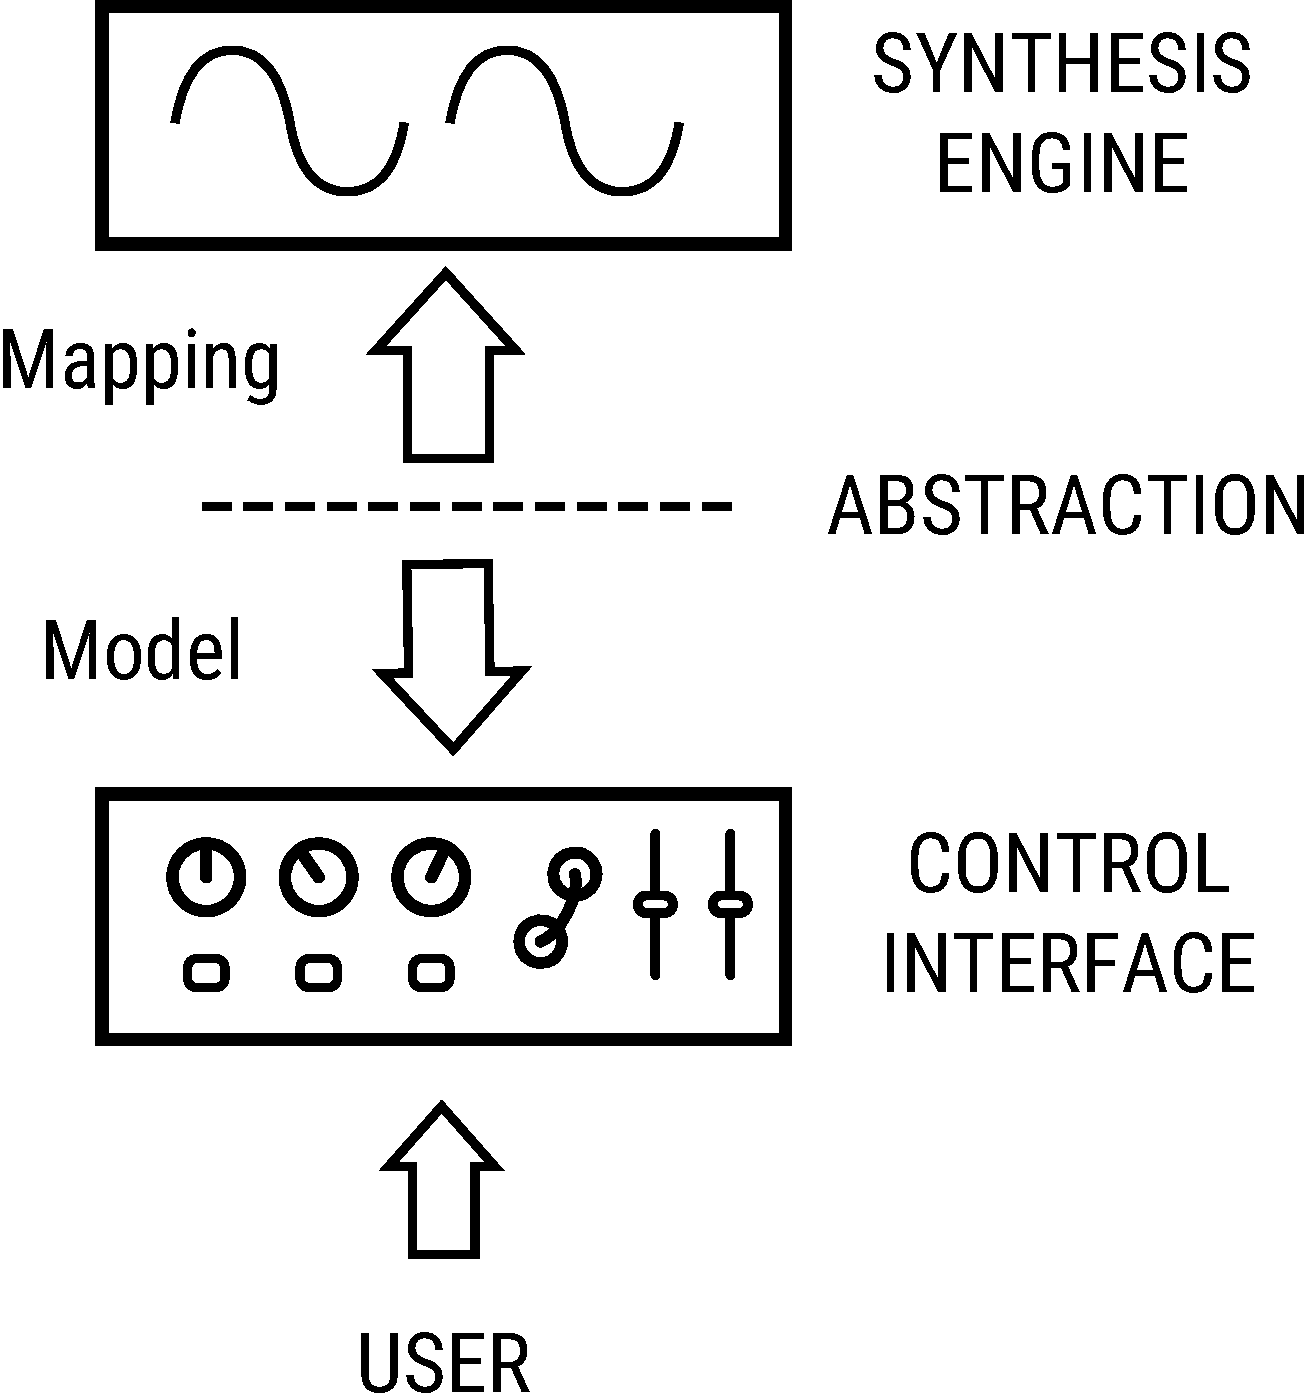
\includegraphics[width=0.4\textwidth]{figures/background/Synth Abstraction Model.pdf}
    \caption{Abstraction between the synthesis engine and control interface. A control interface on a synthesizer is responsible for presenting a conceptual model of the underlying synthesis engine to a user. The parameters on the control interface are mapped back to the synthesis engine to modify audio generation.}
    \label{fig:synth_abstraction}
\end{figure}

\subsection{Synthesis Engine}
The synthesis engine is at the heart of sound generation in any synthesizer, whether it is an analog modular synth or a software audio plugin. Sam McGuire and Nathan Van der Rest provide an overview of the more popular synthesis methods in their book \textit{The Musical Art of Synthesis} \cite{mcguire2015musical}. Popular synthesis methods include the following: subtractive, sample-based, modulation (e.g. FM), additive, wavetable, granular, vector, and physically modelling. 

The exact technique that each synthesis method uses may differ; however, there are common components across many different techniques. It is useful to take a modular perspective when thinking about different synthesizer components, similar to the \textit{unit generator} concept introduced by Max Mathews \cite{roads1980interview}. From this perspective, different components of a synthesizer are broken down into functional units (modules) that can be interconnected in various ways to build up a full synthesizer. We can generalize modules as both producing some output signal and having an optional input signal. Modules may also have parameters that can be mapped to a control interface for user control. We can broadly categorize the signals that are output by modules as either audio signals or control signals. Audio signals are generated by the synthesizer and are ultimately output as a sound. Control signals are used to modulate the parameters of other modules within a synthesizer.

\subsubsection{Types of Modules}
We can further categorize modules into two different types based on the type of signal they output: 1) \textbf{audio modules}, generate or process audio signals, and 2), \textbf{control modules}, generate or process control signals. In analog synthesis, audio signals are commonly generated by voltage-controlled oscillators (VCOs). The frequency of the oscillator in a VCO is controlled by the voltage of an input control signal. While voltages only exist in analog circuits, the concept has been extended into digital synthesizers as well, with the digital equivalent of a VCO sometimes being referred to as a digitally controlled oscillator (DCO). Other common audio modules are voltage-controlled filters (VCFs), voltage-controlled amplifiers (VCAs), and noise sources. Filters accept audio signals as input and attenuate, or boost, specific frequencies, VCAs are essentially an automated volume knob, and noise sources generate different types of noise, such as white noise.

Two common control modules are envelope generators (EGs) and low frequency oscillators (LFOs). Envelope generators are generally triggered in response to an event, for example,  a keyboard note being pressed. Once an EG has been initiated, it produces a control signal that evolves over time. The most common EG is an attack-decay-sustain-release (ADSR) envelope, which was designed to emulate the temporal evolution of instrumental sounds.  %A typical ADSR follows rises to a peak level over a period over time defined by the attack, then falls to a level defined by the sustain over a period of time defined by the decay, stays at the sustain level until the keyboard press is released, and the finally falls back to zero over a period of time defined by the release.
LFOs function the same as regular oscillators, but at a frequency below the threshold of hearing. One common way that LFOs are used is to modulate the pitch on a VCO to create vibrato.

\subsubsection{Subtractive Synthesis}
Subtractive synthesis was one of the earliest methods and is used in Moog synthesizers. The basic idea behind subtractive synthesis is to start with a harmonically rich waveform and subtract from it using filters. This method is associated with the east coast synthesis philosophy. 
%There are several types of waveforms that are generally available on a oscillator in a subtractive synthesizer, these are shown in figure X [insert a diagram of some of the common waveforms and their harmonics]. Each waveform has a unique set of harmonics. Harmonics refer to frequencies that are present in the sound that occur at integer frequency ratios to the fundamental frequency of the sound, which is associated to the perceived pitch of that sound. Sine waves are the simplest waveforms and only contain energy at the fundamental frequency. Noise generators produce energy at all frequencies and contain no fundamental frequency and are therefore inharmonic.

% Once a waveform has been generated it may be combined with other waveforms through a process called mixing. The average subtractive synthesizer has three oscillators \cite{russ2012sound} that are typically tuned to harmonically related frequencies. The next common stage in a subtractive synth signal path is an audio filter. As previously mentioned, one of the most famous synthesizer filters of all time is the Moog ladder filter \cite{moog1965voltage}, which is a resonant low pass/high-pass filter. Low pass filters allow low frequency sounds to pass through while attenuating frequencies above a certain threshold frequency, vice-versa for high-pass filters. The threshold frequency is usually controllable and can be modulated using other signals to create dynamic 'sweeping' sounds. After passing through the filter the signal passes through an amplitude gate, which acts as a volume knob that is controlled by an internal control signal envelope. The envelope 

\subsubsection{Frequency Modulation Synthesis}
FM synthesis engines are capable of producing a huge array of complex waveforms using a relatively simple structure, which makes them powerful; however, they are more conceptually challenging to understand compared to subtractive methods. The basic unit of an FM synthesizer is referred to as an operator, which generally contains a single simple sine wave oscillator and an amplitude gate controlled by an envelope generator. The simplest FM synthesizer consists of two operators that are connected together so that one of the operators controls the frequency of the second operator. The operator that does the modulating is referred to as the \textit{modulator} and the operator that is modulated is referred to the \textit{carrier}. Contrary to subtractive synthesis, FM synthesizers start with simple waveforms and build up to a final timbre using modulation. This method is more associated with west coast synthesis philosophy.

\subsection{Control Interfaces}
\label{sec:control_interfaces}

The control interface of a synthesizer allows a user to build up a conceptual model of the underlying synthesis engine so that they can exert control over the sound being generated. Most synthesizers have interface components such a knobs and sliders that allow users to control the pitch, loudness, and timbre of a generated sound. Keyboard type interfaces and MIDI keyboard controllers provide a direct and easily understood method for controlling pitch for those who are familiar with Western music traditions. Volume controls also provide a relatively direct method for controlling the loudness. The rest of the parameters on a synthesizer control interface are dedicated to controlling the timbre. Seago \cite{seago2004critical} conducted an analysis on synthesizer interfaces and describes three types:
\begin{enumerate}
    \item Parameter selection on a fixed architecture
    \item Architecture specification and configuration
    \item Direct specification of physical characteristics of sound
\end{enumerate}

% Add some images in here for some of the different interface types
Parameter selection interfaces present the user with an organization of synthesizer modules that have been wired together in a fixed arrangement. Generally parameters are arranged in a hierarchical or structured way so as to represent the signal flow of the synthesizer architecture. These are the most common types of interfaces and were the type used on some of the early commercially successful units including the Moog Minimoog (see figure \ref{fig:minimoog}). A majority of software synthesizers emulate fixed architecture synthesizers and many software synthesizers directly emulate hardware interfaces.

\begin{figure}[ht]
    \centering
    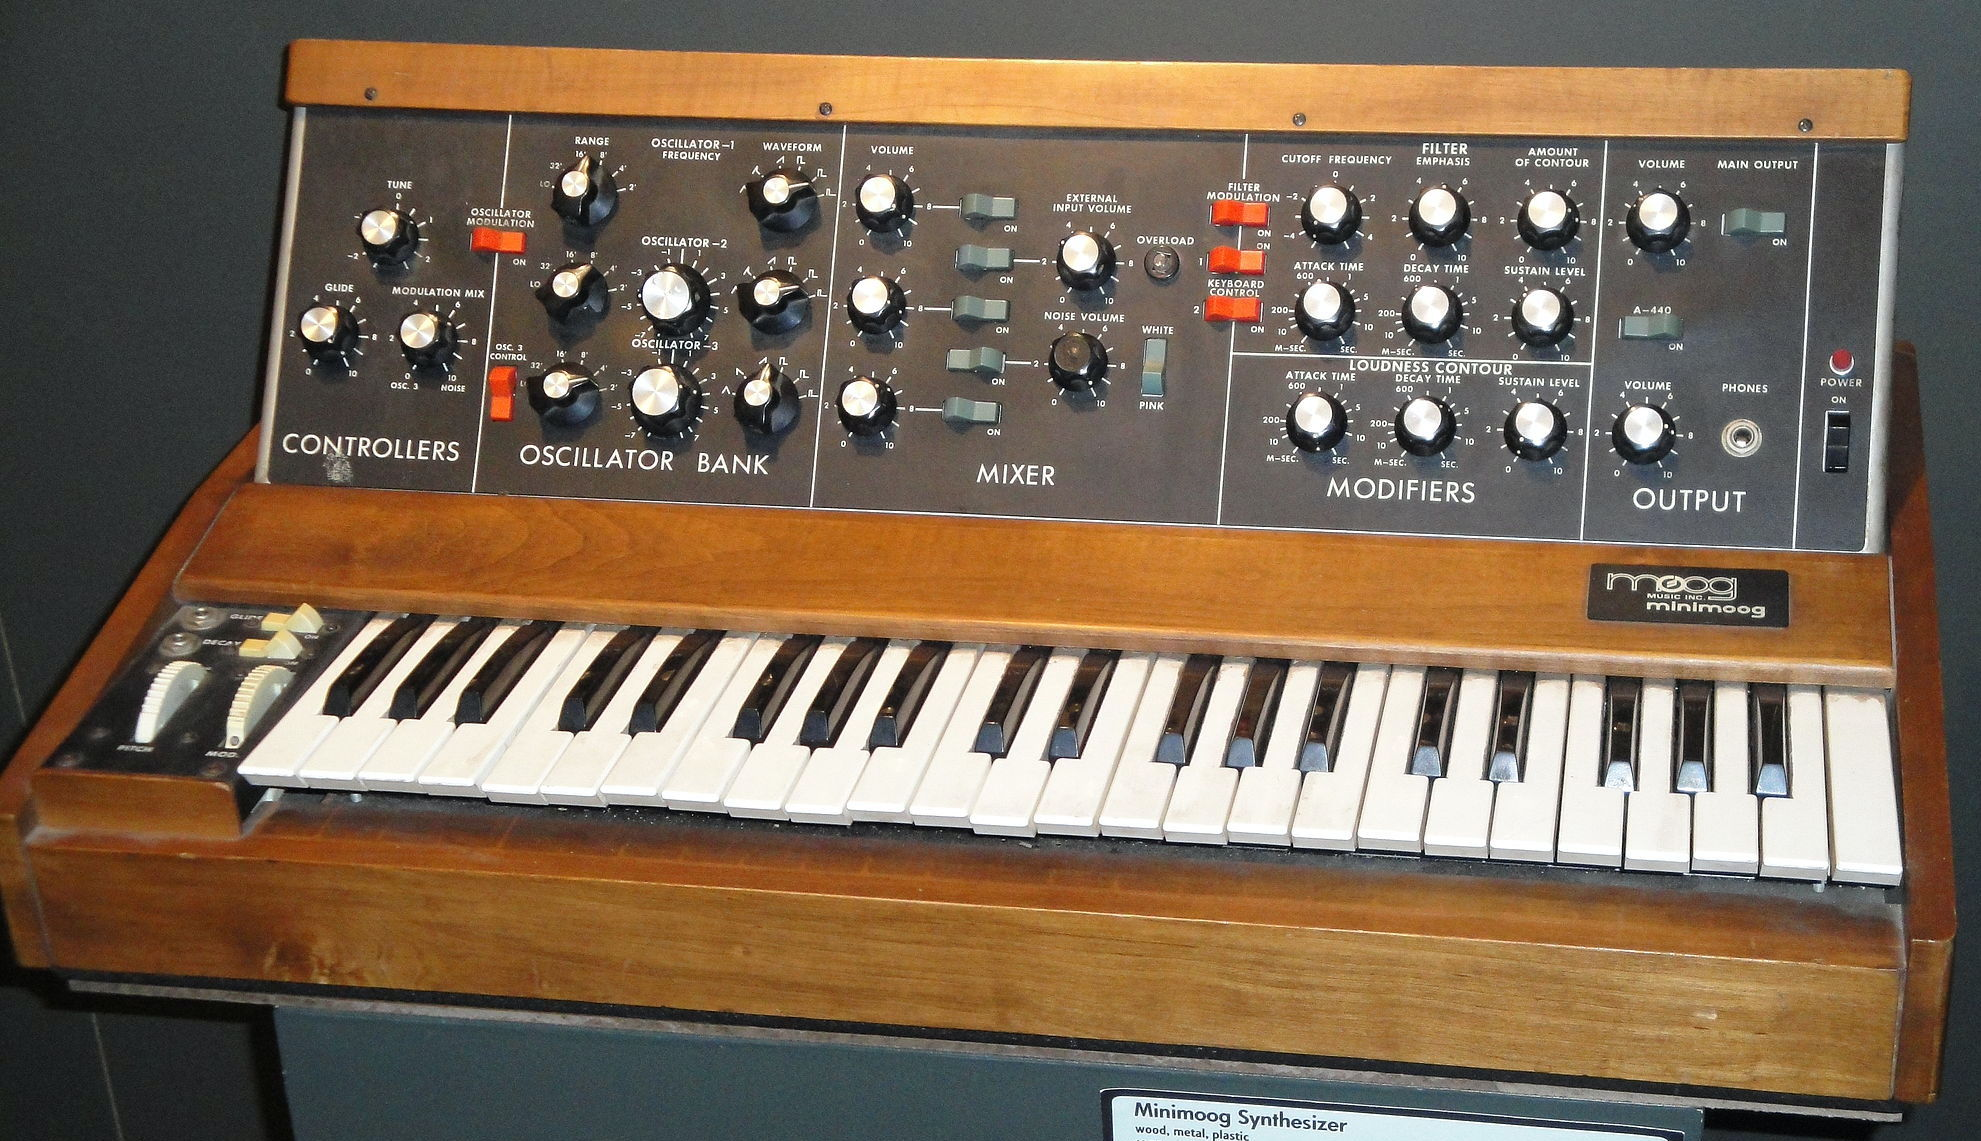
\includegraphics[width=0.8\textwidth]{figures/background/minimoog.jpeg}
    \caption{MiniMoog. An example of a parameter selection on a fixed architecture interface. Photo attribution \cite{harden2009minimoog}.}
    \label{fig:minimoog}
\end{figure}

Architecture specification interfaces allow the user to wire together synthesizer modules. Modular synthesizers are a good example of these types of interfaces. Software like VCV Rack\footnote{\url{https://vcvrack.com/}} provide emulations of Eurorack \cite{intellijel2019} hardware modular synthesizer modules in software (see figure \ref{fig:vcv_rack}). Cycling 74's Max/MSP\footnote{\url{https://cycling74.com/products/max}} and Native Instrument's Reaktor\footnote{\url{https://www.native-instruments.com/en/products/komplete/synths/reaktor-6/}} are other examples of architecture specification interfaces implemented in software.

\begin{figure}[ht]
    \centering
    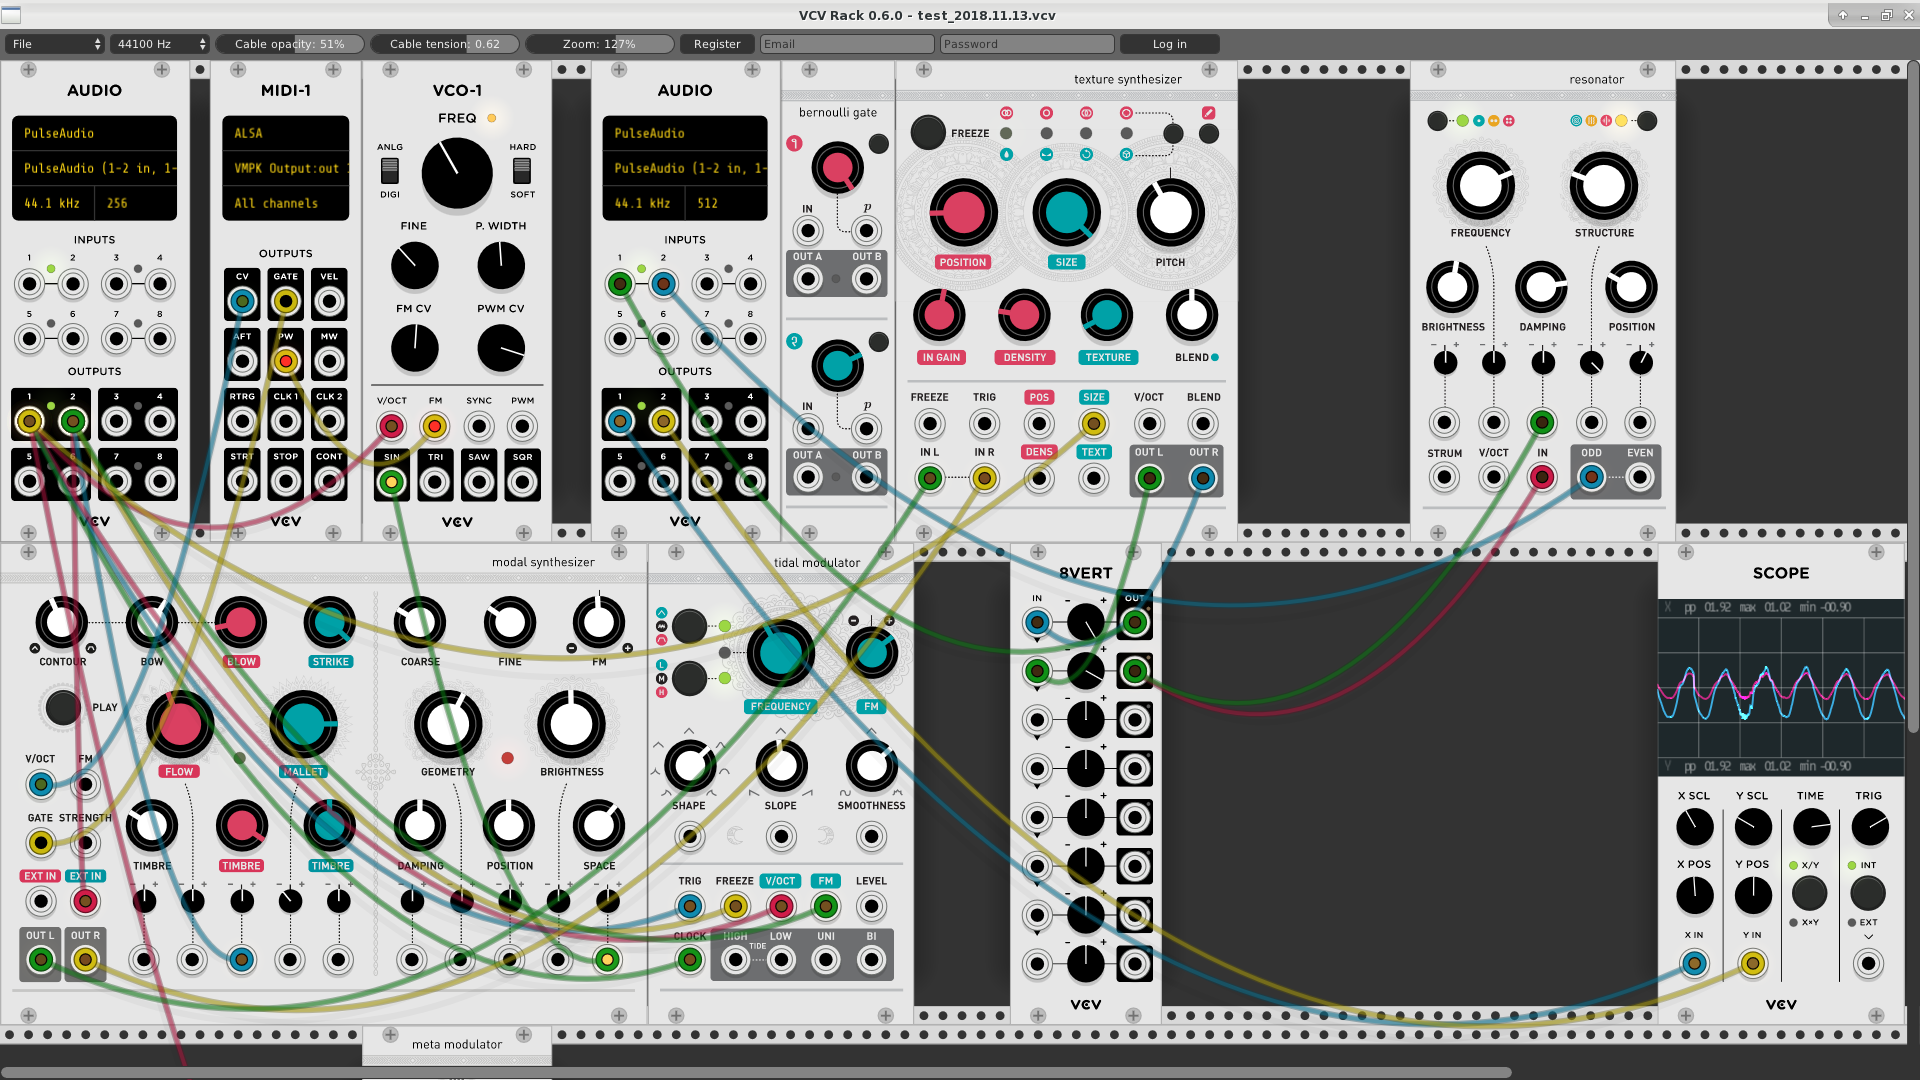
\includegraphics[width=0.8\textwidth]{figures/background/vcv_rack.png}
    \caption{VCV Rack interface. Software synthesizer interface that emulates eurorack modular synthesizers. This is an example of an architecture specification and configuration interface. Photo attribution \cite{popolon2018vcv}.}
    \label{fig:vcv_rack}
\end{figure}

Direct specification interfaces make an attempt to allow the user to interact with the sound itself, as opposed to interacting with a conceptual model of a sound engine. A visual representation of sonic material is presented, typically as the time-domain waveform or a representation of the frequencies. Users are able to draw-in and shape the output sound through this visual interface. This type of interaction can be challenging to use due to the complex relationship between the visual representation of a sound and its perceptual quality. Some software synthesizers provide users a form of direct specification within a larger more traditional architecture: Xfer Records Serum\footnote{\url{https://xferrecords.com/products/serum}} allows users to draw in custom waveforms for wavetables and Izotope Iris\footnote{\url{https://www.izotope.com/en/products/iris.html}} has a visual interface to draw in the frequencies of a spectral filter, shown in \ref{fig:izotope_iris}. 
%\cite{knees2016searching} -- mental images. (this maybe goes into the automatic synthesizer programming section on academic work.

\begin{figure}[ht]
    \centering
    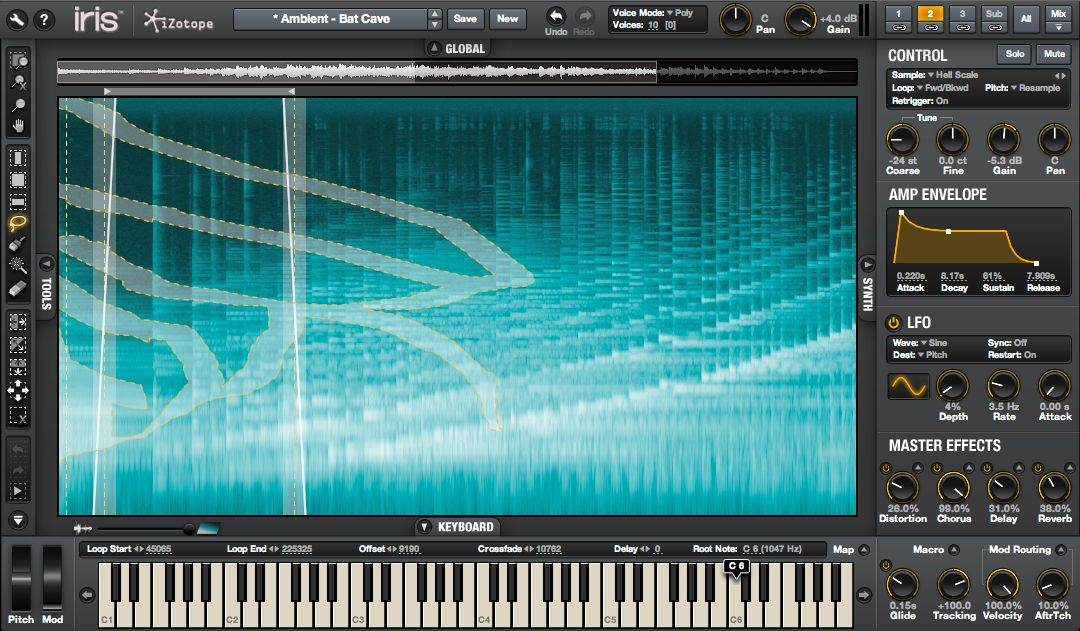
\includegraphics[width=0.80\textwidth]{figures/background/izotope_iris.jpg}
    \caption{Izotope Iris. A sample-playback synthesizer plugin with a visual interface that allows users to draw in frequencies.}
    \label{fig:izotope_iris}
\end{figure}

\subsubsection{Skeumorphism}
A common trend in software synthesizer control interface design is the use of skeumorphism. Skeumorphic interfaces are computer user interfaces that attempt to directly mimic their real-world counterpart. Development of these types of interfaces has become common in audio, partly due to nostalgia of analog audio gear \cite{stuhl2014reactions}. The Arturia Mini V\footnote{\url{https://www.arturia.com/products/analog-classics/mini-v/media}} is an example of a software synthesizer plugin that utilizes skeumorphism. The Mini V emulates the previously mentioned Moog Minimoog. Figure \ref{fig:minimoog_arturia} shows a screenshot of the Arturia Mini V, refer back to figure \ref{fig:minimoog} to see the similarities. Many software synthesizer plug-ins use skeumorphic interfaces, despite the ability for developers to create more nuanced and flexible user interfaces using computer graphic user interfaces (GUIs). %For example [include an image of minimoogs both in hardware and in software].
Researchers have begun to question whether or not these skeumorphic interfaces enhance or hinder usability of audio software \cite{lindh2018beyond}. 

\begin{figure}[ht]
    \centering
    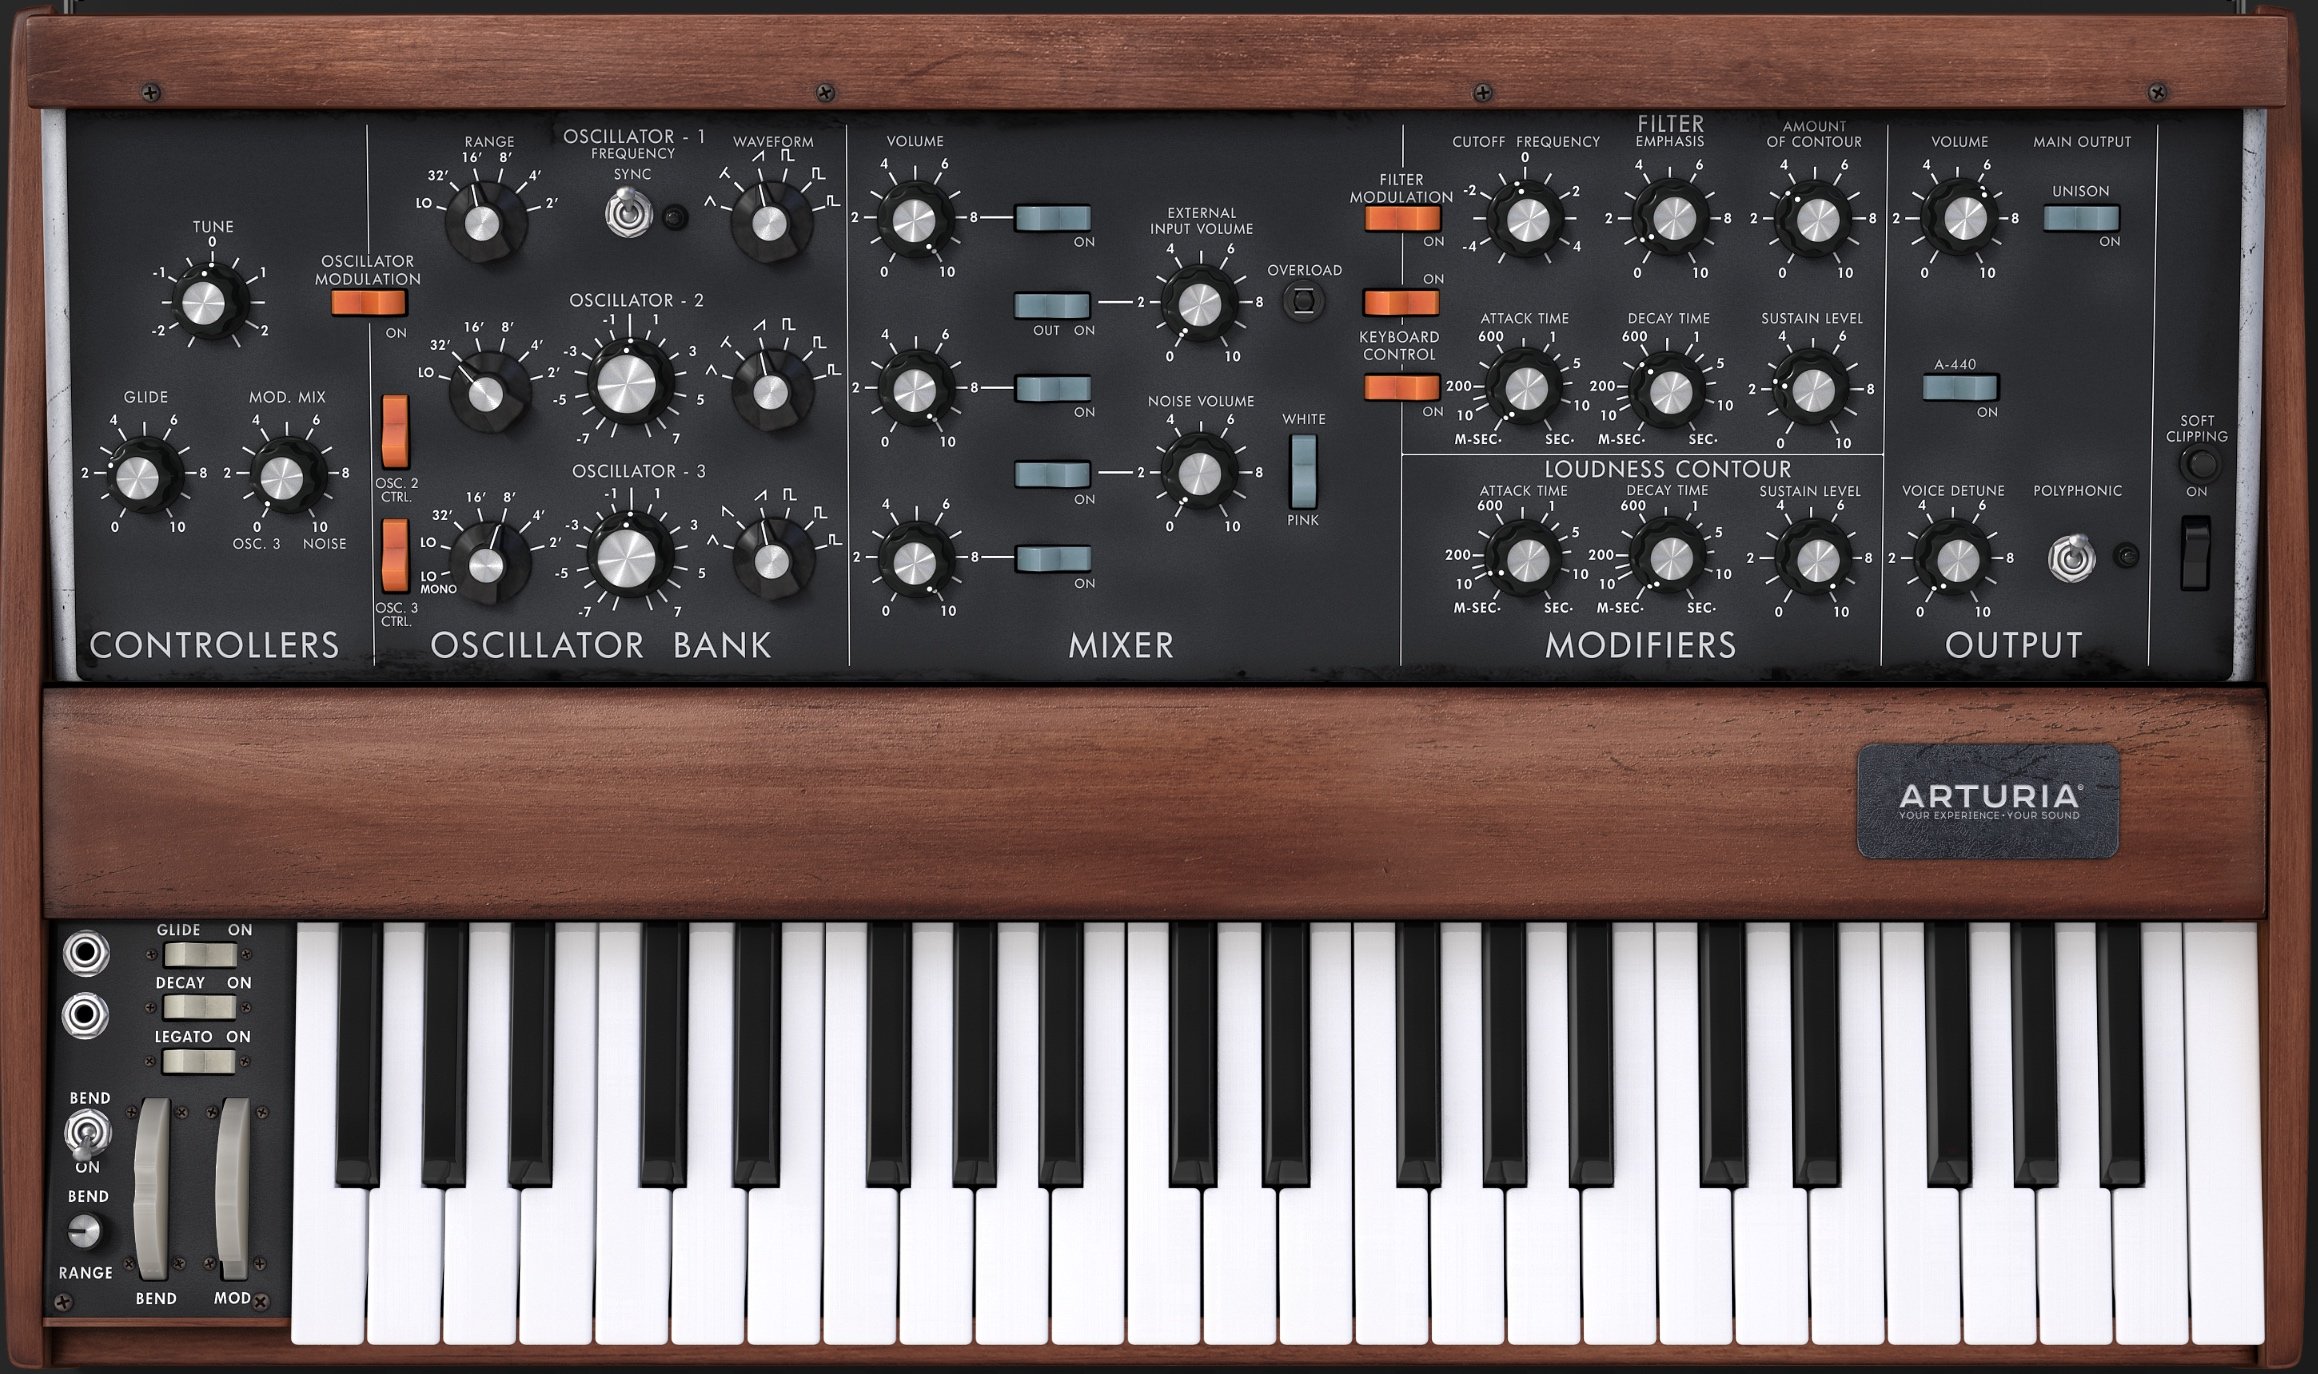
\includegraphics[width=0.7\textwidth]{figures/background/minimoog_arturia.jpg}
    \caption{Arturia Mini V. A software synthesizer plugin emulation of the classic Moog Minimoog synthesizer. The user interface replicates the hardware version as closely as possible, an example of skeumorphic design.}
    \label{fig:minimoog_arturia}
\end{figure}

% Not all software synthesizers utilize skeumorphism and many have introduced new structured methods for organizing the UI onto different pages or subsections that would not be possible on a physical device. One aspect of all control interfaces that is almost universal between hardware and software synthesizers is the use of "knobs", "faders", and other physical controls as parameters. Even though turning a knob with a mouse is quite an awkward interaction, this paradigm is pervasive.

% Not so sure about this section.
% The nature of the control interface is guided by the synthesis method being used by the engine. Synthesis methods like subtractive synthesis which involve a clear linear signal flow that starts with a complex waveform that is progressively shaped can lead to a more simple conceptual model. Moog synthesizers are examples of subtractive synthesizers that have clear control interface that maps to the synthesis engine. More complex synthesis methods such as Frequency Modulation (FM) synthesis are more challenging to create clear control maps for. Interestingly, the most commercially successful synthesizer, the Yamaha DX7, had a notoriously difficult control interface, although shipped with an extensive high-quality set of factory presets (pre-defined control interface parameter settings).


% Bounce this out to another section I think. This could sit in creativity support potentially?
% \subsubsection{Neural Synthesis}
%One area of new development in audio synthesis is in methods that are leveraging advancements from the field of deep learning [deep learning cite], an area of audio synthesis that is explored in this thesis.  
% In contrast to traditional synthesis, neural synthesizers generate audio using large-scale machine learning architectures with millions of parameters \cite{engel2017neural}. Differentiable digital signal processing \cite{engel2020ddsp} bridged the gap between traditional DSP synthesizers with the expressiveness of neural networks, exploring a harmonic model-based approach, using a more compact architecture with 100K parameters.
% One benefit of synthesized audio is that the underlying factors of variation ({\em i.e.}~the parameters) are known.

% % GANs for synthesis
% In this work, we use Generative Adversarial Networks (GANs) \cite{goodfellow2014generative} to generate new instrumental audio from a dataset of existing material. GANs have the potential to be used to generate new sounds on the fly. This would dramatically alleviate both the problem of having to pore through giant sound libraries, and the problem with having to only use one sample repeatedly. In addition, the explosion of new sounds which could potentially be produced by GANs would vastly reduce recording costs by designers of sound libraries.

% This research avenue is to a certain degree untapped: GANs have been successfully applied to the generation and manipulation of images, however, relatively little work has been focused on the audio domain. Research related to the specific work proposed here was presented by \cite{donahue2018adversarial}  and \cite{engel2018gansynth}.
%\cite{ccakir2018musical} - not totally sure what this is about, I think it is generative though.

\section{Synthesizer Programming}
\label{section:synth-programming}

When trying to obtain a particular sound using a synthesizer, users generally have two options: they can try to build up the sound from scratch by adjusting parameters, or they can hope that someone else has gone through that process for them and search through a database of presets to find a sound that fits their criteria. Many users use a preset as a starting point and then manually adjust parameters to reach a desired sound \cite{krekovic2019insights}. The act of programming a synthesizer refers to the process of manually adjusting parameters, whether from scratch or using a preset as a starting point. Synthesizer programming is not an easy task, requiring a strong technical understanding of the particular synthesizer. Carlos and Tomita were masters at programming rich sounds that enhanced their music, and is one of the reasons their work achieved critical acclaim \cite{jenkins2019analog}. Specific techniques for programming synthesizers have lead to the creation of sounds that have defined genres of music, especially in electronic music, such as the ``wobble bass" characteristic of Dubstep and or ``squelchy" synth lines of Acid House tracks. 

%[Maybe need another sentence or so connecting]

% The remainder of this section expands on the challenges associated with synthesizer program to further develop the research motivation, and then finishes with some opportunities for future work that have been identified through user studies and serve as a guide through this work.

\subsection{Challenges}
The difficulty of synthesizer programming was identified in 1979 by James Justice \cite{justice1979analytic}. Justice identified the complexity of real-world sounds and how challenging it is to specify synthesis parameters to recreate sounds in a satisfying way. Richard Ashley later pointed out that the difficulty of synthesizer programming is ``due to the conceptual distance many musicians find existing between their intuitive notions of timbres and the control of synthesis parameter" \cite{ashley1986knowledge}. In more recent work, Pardo \textit{et al.} also describe the challenges of working with audio production tools as being related to the conceptual distance between intuitive spaces and control parameters. 

\subsubsection{Conceptual Spaces of Synthesizer Programming}
There are three conceptual spaces that a user must navigate when using a synthesizer: 1) the parameter space, 2) the perceptual space, and 3) the semantic space. The parameter space represents the control interface and technical aspects of synthesizer programming, e.g. the specific value in Hertz of a filter cutoff. The perceptual space is related to the actual sound of a synthesizer and the semantic space is related to how one would describe the sound, e.g. that sound is ``bright" or ``gritty". When programming a synthesizer, a user must learn to relate between the low-level parameter space and the high-level perceptual / semantic spaces. The relationship between the low-level and high-level spaces is often complex. This complexity is responsible for the ``conceptual distance" that Ashley was referring to \cite{ashley1986knowledge}. Figure \ref{fig:synth_conceptual_dist} shows an updated version of the synthesizer diagram from \ref{fig:synth_abstraction} with the conceptual distance between the parameter space and the perceptual space. Users must translate desired auditory changes (the perceptual space) to modifications in the control interface (the parameter space).

\begin{figure}[ht]
    \centering
    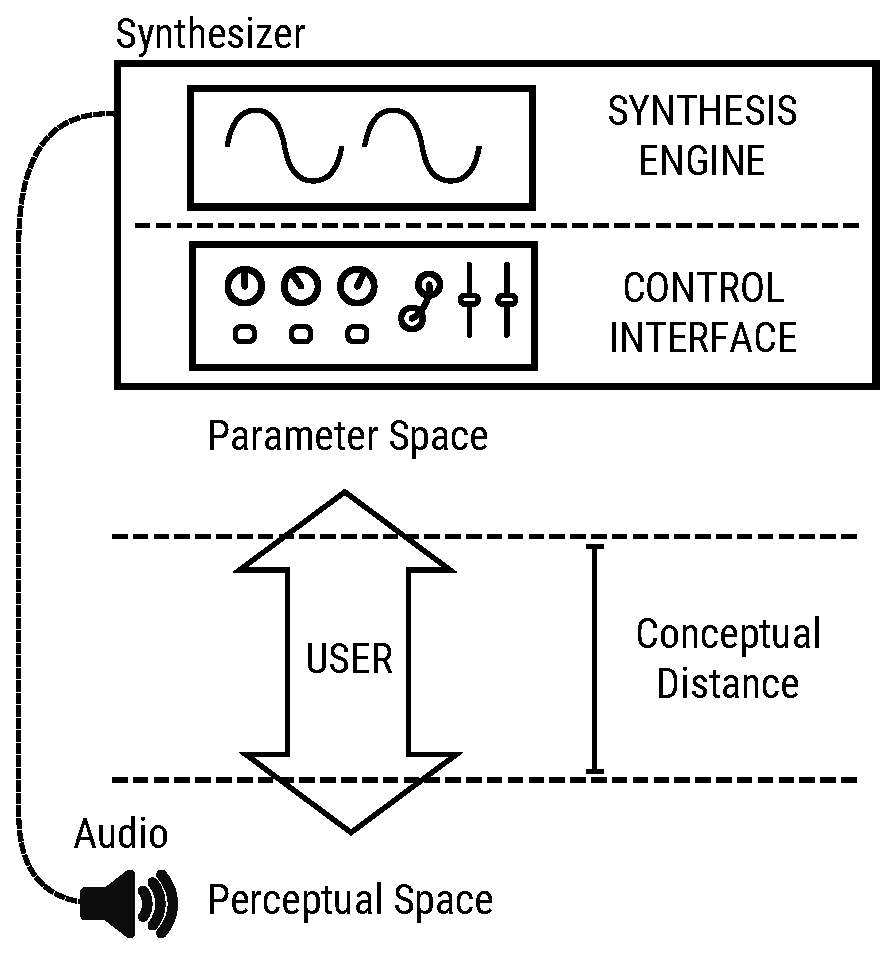
\includegraphics[width=0.5\textwidth]{figures/background/synth_conceptual_dist.eps}
    \caption{Updated figure of the components of a synthesizer (from figure \ref{fig:synth_abstraction}) showing the conceptual distance between the parameter space and the perceptual space that the user must translate between.}
    \label{fig:synth_conceptual_dist}
\end{figure}

\subsubsection{Specifying Timbre}
Perception of musical tones can be described as being comprised of three dimensions: pitch, loudness, and timbre. Synthesizers typically have controls for specifying all three of these dimensions. Pitch and loudness are uni-dimensional and have relatively simple mappings to parameters \cite{seago2004critical}. Therefore, the vast majority of parameters, which can be over hundred, are used to specify timbre. This means that the core of problem of synthesizer programming resides in the mapping between the perceptual and semantic spaces of timbre and the space of synthesizer parameters.
 
Following this, developing a good understanding of how timbre is defined would be a good place to begin to learn how to build more intuitive synthesizer controls. Unfortunately, we are at once faced with a challenge. The ANSI definition describes timbre as the attribute of auditory sensation that allows one sound be distinguished from other sounds at the same pitch and loudness \cite{american1973american}. This definition doesn't tell us very much about what timbre is, as opposed to what it is not. Understanding precisely what musical timbre \textit{is} has presented itself as challenging problem \cite{krumhansl1989musical} and significant research has been conducted to try to answer this. McAdams identifies that timbre is a purely perceptual quality of sound and provides a review of the subject \cite{mcadams2019}. In early research on musical timbre, Grey described timbre as being multi-dimensional and introduced the concept of a three dimensional \textit{Timbre Space} \cite{grey1977multidimensional}. Risset and Wessel explore timbre in the context of sound synthesis and emphasize the spectro-temporal representation of sound for understanding timbre \cite{risset1999exploration}. This conception of timbre stresses the importance of the temporal aspects of sound and how the various frequency components of a sound evolve over time to our perception of timbre. More recent research based on neuroscience is moving away from the idea that timbre comprises a set of unique dimensions, but is instead a complex high-dimensional quality that must be taken as a whole \cite{mcadams2019}. 

All this is to say that deriving a concrete definition for timbre in the context of an audio synthesizer is a complicated problem. The intractable nature of the problem is one of the main reasons that the conceptual distance between the perceptual / semantic space of a synthesizer and the parameter space is so large. Defining parameters in technical terms based on their relation to the synthesis engine is a much more precise and concrete way to design a control interface, so it is not surprising that is what the vast majority of synthesizer developers do. Unfortunately, this means that users are stuck with learning the technical domain language of a particular synthesizer and learning to relate that to their own perceptual / semantic conception of the associated audio output.

\subsubsection{Impediments of Synthesizer Programming}
Gordan Krekovi\'{c} recently conducted a study with synthesizer users that provides insight into attitudes towards synthesizer programming \cite{krekovic2019insights}. 122 individuals participated in that study, which consisted of answering questions related to their experiences with synthesizers. A majority of users were very experienced with synthesizers, 71\% had ten or more years of experience, and only 2.7\% were novice users, having less then a few months of experience. Krekovi\'{c} identified four impediments of synthesizer programming and asked the participants how much they agreed with each impediment:
\begin{enumerate}
    \item it can be time consuming;
    \item it can be a distraction from focusing on music;
    \item it can be difficult and non-intuitive to learn to use a particular instrument;
    \item it rarely leads to desirable results.
\end{enumerate}
Most participants agreed with statements 1-3 and disagreed with statement 4, however, participants with less experience were more likely to agree with statement 4. This indicates that users with more experience programming synthesizers more often felt that they were able to achieve desirable results. The fact that most participants agreed with statements 1-3, especially given that the majority are highly experienced synthesizer users, indicates the extent of the challenges associated with synthesizer programming. Even after ten years of experience, users still feel like synthesizers can be difficult and non-intuitive to use. When given the opportunity to write about their experiences in a more open-ended way, participants generally reported on difficulties with user-interfaces, learning specific synthesizers, limited features, and the creative process.

\subsubsection{Differences between Synthesizers}
As mentioned earlier, there are a large number of different approaches to synthesis, and even within a particular synthesis type (e.g., subtractive or FM) there could be a nearly infinite number of variations. This is reflected by the hundreds of different software synthesizers that are currently commercially available on websites like KVR\footnote{\url{https://www.kvraudio.com/plugins/softsynth-virtual-instruments}}. Some methods such as subtractive synthesis have parameters that are more intuitively understood, whereas methods like FM synthesis ``may be viewed as essentially an exploration of a mathematical expression, but whose parameters have little to do with real-world sound production mechanisms, or with perceived attributes of sound" \cite{seago2013new}. These challenges and their affect on synthesizer programming is summarized in one of the responses from Krekovi\'{c}'s study:

\begin{quote}
    Different sorts of synthesis require different background knowledge, most of which have steep learning curves that are at least partially exclusive. In other words, there is an enormous investment of time to deeply learn how the different forms of synthesis work. This learning is a prerequisite to effective use of synthesizers.
\end{quote}

% \subsubsection{Software Synthesizers}

% Not sure exactly how to make this section work.

% Bates had some good stuff on challenges specific to software synthesis.
% Products such as these expanded the field of musicians who were attracted by the possibilities of allegedly limitless sound design and creative production, but the unwieldy user interfaces of softsynths, which depended almost exclusively on user mouse clicking on skeuomorphic visual representations of hardware gear alongside complex “menu diving” scenarios, made for an extremely frustrating and kinesthetically/haptically nonmusical user experience.


% When conducting an analysis on the usability of synthesizers and the affect that has on synthesizer programming, it is easy to take on the perspective that any challenge is negative and must be eradicated. There is, however, indication that users enjoy the complexity of synthesizers and the challenges of programming. This is illustrated by the recent resurgence in hardware modular synthesizers. Modular synthesizers are more complicated and time-consuming to use than software synthesizers for a number of reasons, and are more likely to lead to unsatisfactory results, yet the demand for them has shot up in recent years \cite{bates2021interface}. This points to realization that programming a synthesizer, despite it being challenging and time-consuming, is an enjoyable experience and something worth doing regardless of the quality of the final result.

% Bates attributes 


% In fact, research in the field of music interaction \cite{holland2013music} highlights the importance of challenges in creating an engaging musical experience and questions the benefit of making music interaction easy \cite{mcdermott2013should}.

% Results from Krekovi\'{c}'s study point to this as well, despite the fact that participants agreed with three out of four of the impediments, they still chose to manually program more often than not, and most had for many years. This conclusion could of course be drawn based on survivor bias: the users who participated in the study hadn't given up with synthesizer programming in the face of the challenges; they either enjoyed it enough, or had another good reason, to keep going despite the impediments. 

% The question arises, how many potential synthesizer users are not represented because they never made it past the initial learning curve? 

\subsection{Opportunities}
Based on the pervasiveness of the identified challenges and complexities associated with synthesizer programming, there is opportunity for development of methods that support both novices and experts. In fact, research into approaches that help bridge the conceptual gap between the perceptual / semantic and parameter spaces of synthesizers has been ongoing for over 40 years now. This research broadly falls under the umbrella of automatic synthesizer programming and will be reviewed in-depth in the next chapter.

To inform future work in this area, Krekovi\'{c} asked participants to rate their perceived helpfulness of four proposed systems based on approaches from previous work. The systems proposed were: 1) a system that generates random presets within a category, 2) a user provides a description of a the desired sound and a preset is generated for them, 3) a user provides an example sound and the system generates a presets to sound similar, and 4), more intuitive interactive user interface. Participants thought that proposed systems three and four would be helpful and systems one and two would be slightly helpful.

\section{Summary}
This chapter provided an overview of audio synthesizers and the task of synthesizer programming, which involves manually adjusting parameters to achieve a desired sound. A brief history of the evolution of synthesizers was provided, starting with analog synthesizers and leading up to software synthesizers that are implemented as audio plugins that work directly within modern digital audio workstations. The core of any synthesizer is the synthesis engine, which generates audio using a variety of different possible techniques. Users can control the synthesis engine through a control interface by modifying a potentially large number of parameters. The majority of this process of adjusting parameters, which is referred to as synthesizer programming, is related to the specification of timbre. Three conceptual spaces are involved in the process of synthesizer programming: the perceptual space, semantic space, and parameter space \cite{pardo2019learning}. The perceptual and semantic space are higher level and are more directly understood by humans, whereas the parameter space is technical and relates directly to a particular synthesis algorithm. The distance between the perceptual / semantic space and the parameter space is large and leads to difficulties in learning how to use synthesizers effectively. The affect of these challenges was reflected by users in a recent user study \cite{krekovic2019insights} and opportunities for improvement to current synthesizer programming paradigms was identified. Automatic synthesizer programming has developed to address the challenges associated with synthesizer programming. An overview of automatic synthesis programming is provided in the next chapter.